\documentclass{beamer}
\setbeamerfont{subsection in toc}{size=\footnotesize}
%\setbeameroption{show notes on second screen=left} %enable for notes
\usepackage{graphicx}
\usepackage{xcolor}
\usepackage{listings}
\usepackage{hyperref}
\lstset{language=python,frame=single}
\usepackage{verbatim}
\usepackage[longnamesfirst]{natbib}
\usepackage{subcaption}
\usepackage{amsmath}
\usepackage{bm}
\usepackage{relsize}
\usepackage{appendixnumberbeamer}
\usepackage{xparse}
\usepackage{multimedia}
\usepackage{xcolor}
\usepackage[normalem]{ulem}
\usepackage{hyperref}
\usepackage{pdfpc-commands}
\usepackage{tikz}
\usetikzlibrary{matrix,backgrounds}
\usetikzlibrary{positioning}
\usetikzlibrary{shapes,arrows}
\usetikzlibrary{decorations.pathreplacing, calligraphy}

\captionsetup[subfigure]{labelformat=empty}

\tikzset{onslide/.code args={<#1>#2}{%
  \only<#1>{\pgfkeysalso{#2}} 
}}

\tikzstyle{block} = [rectangle, draw, thick, align=center, rounded corners]
\tikzstyle{boundingbox} = [thick, lightgray]
\tikzstyle{dashblock} = [rectangle, draw, thick, align=center, dashed]
\tikzstyle{conc} = [ellipse, draw, thick, dashed, align=center]
\tikzstyle{netnode} = [circle, draw, very thick, inner sep=0pt, minimum size=0.5cm]
\tikzstyle{relunode} = [rectangle, draw, very thick, inner sep=0pt, minimum size=0.5cm]
\tikzstyle{line} = [draw, very thick, -latex', -]
\tikzstyle{arrow} = [draw, ->, very thick]

\definecolor{bpurp}{HTML}{984ea3}
\definecolor{bblue}{HTML}{377eb8}
\definecolor{bred}{HTML}{e41a1c}

\usetheme[numbering=none]{metropolis}

\begin{document}

\title{Meta-Mapping: Toward human-like flexibility from deep learning}
\author{Andrew Lampinen}
\date{}
\frame{\titlepage}

\begin{frame}<1-3>[label=pokermotivation]
\frametitle<1-4>{Humans are good at adapting flexibly}
\frametitle<5>{Switching to opposite rewards is challenging}
\centering
\only<1>{
\includegraphics[width=\textwidth]{figures/poker.png}
}
\only<2>{
\includegraphics[width=\textwidth]{figures/frostbite.jpg}
}
\only<3>{
\includegraphics[height=0.4\textheight]{../../psych/dissertation/4-extending/figures/categorization_stimuli/32_yellow_inverseplus_1.png}
}
\end{frame}
%% Don't forget to say starting point!!!

\begin{frame}{Deep learning is (usually) not}
\begin{columns}
\begin{column}{0.5\textwidth}
Deep learning generally requires lots of data to achieve good performance on a task. However, there are a few exceptions:
\begin{itemize}[<+(2)->]
    \item Lots of new work on meta-learning (learning to learn), for learning from little data, but not none.
    \item Some language work
    \item Model-based RL. 
    \item I'll discuss these approaches along the way. 
\end{itemize}
\end{column}

\begin{column}{0.5\textwidth}
\includegraphics[width=\textwidth]{figures/poker.png}
\includegraphics[width=\textwidth]{figures/frostbite.jpg}
\end{column}
\end{columns}
\end{frame}

\begin{frame}[standout]
How can we build deep learning models that can perform a new task well on their first try, based on its relationship to prior tasks?
\end{frame}

\section{Meta-mapping}

\begin{frame}{Tasks as functions/mappings}
\begin{columns}
\begin{column}{0.5\textwidth}
It's useful to think of tasks or behaviors as functions mapping input to output:
\begin{itemize}
    \item Poker hand \(\rightarrow\) bet
    \item Chess position \(\rightarrow\) move
    \item Object \(\rightarrow\) classification
\end{itemize}
Standard deep learning tries to infer this mapping from lots of examples. 
\end{column}

\begin{column}{0.5\textwidth}
\includegraphics[width=\textwidth]{figures/poker_function.png}
\end{column}
\end{columns}
\end{frame}

\begin{frame}[standout]
Tasks \(\bm =\) mappings from inputs to outputs. 
\end{frame}

\begin{frame}{Meta-learning}
\begin{columns}
\begin{column}{0.5\textwidth}

\begin{itemize}[<+->]
    \item Lots of recent research on meta-learning -- learning to learn.
    \item If you have learned a lot of card games, you should be able to pick up a new one from a few examples.
    \item Then apply this knowledge to play the game with probe hands you weren't taught. 
    \item But, again, how could we play a variation of the game without examples? 
\end{itemize}
\end{column}

\begin{column}{0.5\textwidth}
\includegraphics[width=\textwidth]{figures/poker_function_2.png}
\end{column}
\end{columns}
\end{frame}

\begin{frame}{Mapping flexibility}
If tasks are mappings, altering the task = adapting the mapping. 
\begin{columns}
\begin{column}{0.5\textwidth}
\vspace{2em}
\includegraphics[width=\textwidth]{figures/poker.png}
\end{column}
\begin{column}{0.5\textwidth}
\vspace{2em}
\only<1>{
\includegraphics[width=\textwidth]{figures/poker_function.png}
}
\only<2>{
\includegraphics[width=\textwidth]{figures/lose_poker_function.png}
}
\end{column}
\end{columns}
\end{frame}

\begin{frame}[standout]
We want to model how we can adapt the task mapping.
\end{frame}

\begin{frame}{Meta-mappings}
How do we get from a task function to an adapted one?
\begin{itemize}
\item We propose \textbf{meta-mappings}, higher-order mappings which transform mappings into other mappings.
\end{itemize}
\includegraphics[width=\textwidth]{figures/meta_mapping_poker.png}
\end{frame}

\begin{frame}[standout]
Transforming the task mapping \(=\) adapting. \\[1em]
Meta-mappings are higher-order mappings that transform task mappings.
\end{frame}

\begin{frame}<-3>[label=basic_metamapping_analogy]
\frametitle{Meta-mappings are analogous to basic tasks}
\begin{columns}
\begin{column}{0.5\textwidth}
\vspace{2em}
\includegraphics[width=\textwidth]{figures/poker_function.png}
\end{column}
\begin{column}{0.5\textwidth}
\vspace{2em}
\includegraphics[width=\textwidth]{figures/try_to_lose_function.png}
\end{column}
\end{columns}
\only<-3>{
\begin{itemize}[<+->]
\item Both are just functions (they just have different types of inputs and outputs).
\item This means we can apply all the usual deep learning tricks to meta-mappings.
\item ... Assuming we have a way to represent the basic tasks for input to (and output from) the meta-mappings. 
\end{itemize}
}
\end{frame}

\begin{frame}[standout]
There is a functional analogy between basic tasks and meta-mappings. \\[1em]
But how can we use it?
\end{frame}

\section{An architecture for representing and transforming tasks}

\begin{frame}{Architecture preview}
Our goal is to implement:
\begin{itemize}
\item A way of representing tasks as mappings.
\item A way of representing those tasks/mappings as vectors.
\item A way of learning to transform those task-vectors to perform meta-mappings.
\end{itemize}
This will allow the architecture to perform new tasks without data, by their relationship to prior tasks.
\end{frame}

\begin{frame}{Task-specific computations are low-dimensional and abstract}
\begin{tikzpicture}[auto]
\node at (-4, 0) (image) {\includegraphics[width=2cm]{figures/straight_flush_hand.jpg}};


%% input

\node[netnode] at (-2.25, -1.5) (i00) {};
\node[netnode] at (-2.25, -0.75) (i01) {};
\node[netnode] at (-2.25, 0) (i02) {};
\node[netnode] at (-2.25, 0.75) (i03) {};
\node[netnode] at (-2.25, 1.5) (i04) {};

\path [line] ([xshift=-3]image.east) to (i00);
\path [line] ([xshift=-3]image.east) to (i01);
\path [line] ([xshift=-3]image.east) to (i02);
\path [line] ([xshift=-3]image.east) to (i03);
\path [line] ([xshift=-3]image.east) to (i04);

\node[netnode] at (-1, -1.5) (i10) {};
\node[netnode] at (-1, -0.75) (i11) {};
\node[netnode] at (-1, 0) (i12) {};
\node[netnode] at (-1, 0.75) (i13) {};
\node[netnode] at (-1, 1.5) (i14) {};

\path [line] (i00) to (i10);
\path [line] (i00) to (i11);
\path [line] (i00) to (i12);
\path [line] (i00) to (i13);
\path [line] (i00) to (i14);
\path [line] (i01) to (i10);
\path [line] (i01) to (i11);
\path [line] (i01) to (i12);
\path [line] (i01) to (i13);
\path [line] (i01) to (i14);
\path [line] (i02) to (i10);
\path [line] (i02) to (i11);
\path [line] (i02) to (i12);
\path [line] (i02) to (i13);
\path [line] (i02) to (i14);
\path [line] (i03) to (i10);
\path [line] (i03) to (i11);
\path [line] (i03) to (i12);
\path [line] (i03) to (i13);
\path [line] (i03) to (i14);
\path [line] (i04) to (i10);
\path [line] (i04) to (i11);
\path [line] (i04) to (i12);
\path [line] (i04) to (i13);
\path [line] (i04) to (i14);

%% task specific
\node[netnode] at (0.25, -0.375) (t00) {};
\node[netnode] at (0.25, 0.375) (t01) {};

\path [line] (i10) to (t00);
\path [line] (i10) to (t01);
\path [line] (i11) to (t00);
\path [line] (i11) to (t01);
\path [line] (i12) to (t00);
\path [line] (i12) to (t01);
\path [line] (i13) to (t00);
\path [line] (i13) to (t01);
\path [line] (i14) to (t00);
\path [line] (i14) to (t01);

\node[netnode] at (1.5, -0.375) (t10) {};
\node[netnode] at (1.5, 0.375) (t11) {};

\path [line] (t00) to (t10);
\path [line] (t00) to (t11);
\path [line] (t01) to (t10);
\path [line] (t01) to (t11);

%% output

\node[netnode] at (2.75, -1.5) (o00) {};
\node[netnode] at (2.75, -0.75) (o01) {};
\node[netnode] at (2.75, 0) (o02) {};
\node[netnode] at (2.75, 0.75) (o03) {};
\node[netnode] at (2.75, 1.5) (o04) {};

\path [line] (t10) to (o00);
\path [line] (t11) to (o00);
\path [line] (t10) to (o01);
\path [line] (t11) to (o01);
\path [line] (t10) to (o02);
\path [line] (t11) to (o02);
\path [line] (t10) to (o03);
\path [line] (t11) to (o03);
\path [line] (t10) to (o04);
\path [line] (t11) to (o04);

\node[netnode] at (4, -1.5) (o10) {};
\node[netnode] at (4, -0.75) (o11) {};
\node[netnode] at (4, 0) (o12) {};
\node[netnode] at (4, 0.75) (o13) {};
\node[netnode] at (4, 1.5) (o14) {};

\path [line] (o00) to (o10);
\path [line] (o00) to (o11);
\path [line] (o00) to (o12);
\path [line] (o00) to (o13);
\path [line] (o00) to (o14);
\path [line] (o01) to (o10);
\path [line] (o01) to (o11);
\path [line] (o01) to (o12);
\path [line] (o01) to (o13);
\path [line] (o01) to (o14);
\path [line] (o02) to (o10);
\path [line] (o02) to (o11);
\path [line] (o02) to (o12);
\path [line] (o02) to (o13);
\path [line] (o02) to (o14);
\path [line] (o03) to (o10);
\path [line] (o03) to (o11);
\path [line] (o03) to (o12);
\path [line] (o03) to (o13);
\path [line] (o03) to (o14);
\path [line] (o04) to (o10);
\path [line] (o04) to (o11);
\path [line] (o04) to (o12);
\path [line] (o04) to (o13);
\path [line] (o04) to (o14);

\node at (5.25, 0) (output) {\textbf{\$\$\$}};
\path [line] (o10) to (output.west);
\path [line] (o11) to (output.west);
\path [line] (o12) to (output.west);
\path [line] (o13) to (output.west);
\path [line] (o14) to (output.west);

%% overlays
\uncover<2->{
\draw[fill=black, opacity=0.2] (-2.9, -3.5) rectangle (-0.25, 2);
\draw[fill=black, opacity=0.2] (2, -3.5) rectangle (4.5, 2);
\draw[fill=red, opacity=0.4] (-0.25, -3.5) rectangle (2, 2);
}

%% anotations

\node at (-4, -3) {\textbf{Input}};
\node[text width=2.5cm, align=center] at (-1.625, -3) {\textbf{Shared ``perception''}};
\node[text width=2cm, align=center] at (0.875, -3) {\textbf{Task specific}};
\node[text width=2.5cm, align=center] at (3.375, -3) {\textbf{Shared ``motor''}};
\node at (5.25, -3) {\textbf{Output}};


\end{tikzpicture}
\end{frame}

\begin{frame}<-2>[label=homm_basic]
\frametitle{A multi-task architecture}
\begin{columns}
\begin{column}{0.5\textwidth}
\begin{tikzpicture}
%% basic meta learning
\draw[boundingbox, fill=white] (-3, -4.3) rectangle (2.5, 3.2);
\node[lightgray] at (-1.2, 2.9) {\only<1>{Deep learning}\only<2->{Meta-learning}};
\node at (-1.5, -4) (examples) {Examples};
\node at (-1.5, -3.2) (D1) {
\(\left\{
\begin{matrix}
(x^{ex}_{in,0}, y^{ex}_{targ,0})\\
$\vdots$
\end{matrix}\right\}\)};

\node at (1.5, -4) (probes) {Probes};
\node at (1.5, -3.2) (D2) {
%\(z^{prb}_{in}\)};
\(\left\{
\begin{matrix}
x^{prb}_{in,0}\\
$\vdots$
\end{matrix}\right\}\)};

\uncover<2->{
\node [block] at (-1.5, -1.95) (M) {\(\mathcal{M}\)};
\path [arrow] ([yshift=-5]D1.north) to (M);

\node at (-1, -1) (zfunc) {\(z^{task}\)};
\path [arrow, out=90, in=-135] (M.north) to ([xshift=6,yshift=3]zfunc.south west);

\node[block] at (0, -0.55) (H) {\(\mathcal{H}\)};
\path [arrow, out=45, in=180] ([yshift=-3]zfunc.north) to (H.west);
}
\node [block, dashed] at (1.5, -0.55) (F) {\(F_{z^{task}}\)};
\uncover<2->{
\path[arrow] (H.east) to (F.west);
}
\path [arrow, dashed] (D2) to (F);

\node at (1.5, 1) (outputs) {
%\(z^{pred}_{out}\)};
\(\left\{
\begin{matrix}
y^{pred}_{out,0},\\
$\vdots$
\end{matrix}\right\}\)};
\node at (1.5, 1.8) (predictions) {Predictions};

\path [arrow, dashed] (F) to ([yshift=3]outputs.south);

\node at (-1.5, 1.8) (probetargs) {Probe targets};
\node at (-1.5, 1) (D2targs) {
%\(z^{prb}_{in}\)};
\(\left\{
\begin{matrix}
y^{prb}_{targ,0}\\
$\vdots$
\end{matrix}\right\}\)};

\node [align=center, text width=1.25 cm] at (0, 2.25) (dispatch) {\baselineskip=12pt Loss\par};

\path [arrow, dashed, out=180, in=-90] ([xshift=3]outputs.west) to (dispatch.south);

\path [arrow, dashed, out=0, in=-90] ([xshift=-3.5]D2targs.east) to (dispatch.south);

%% overlay

\draw [fill=black, opacity=0.2] (0.75, -0.2) rectangle (2.25, 0.35);
\draw [fill=red, opacity=0.4] (0.75, -1) rectangle (2.25, -0.2);
\draw [fill=black, opacity=0.2] (0.75, -2.5) rectangle (2.25, -1);

\uncover<4->{
\draw [red, ultra thick] (-1, -1) circle (0.5);
}
\end{tikzpicture}
\end{column}
\begin{column}{0.5\textwidth}
\includegraphics[width=\textwidth]{figures/poker_function_2.png}
\end{column}
\end{columns}
\end{frame}

\begin{frame}[standout]
We use an architecture which generates task embeddings from examples and uses these embeddings to parameterize (part of) a deep network which performs the task. % shorten this
\end{frame}

\againframe<4>{homm_basic}

\begin{frame}<1>[label=homm_arch]
\frametitle<1>{Meta-mapping as transforming function embeddings}
\frametitle<2>{So we can use the same approach and networks!}
\frametitle<3>{Language-based approach}
\frametitle<4>{Language-based meta-mapping}
\begin{columns}
\begin{column}{\dimexpr\paperwidth-10pt}
\centering
\begin{tikzpicture}[scale=0.7, every node/.style={scale=0.7}]
%% basic meta learning
\begin{scope}[shift={(0.4, 0.4)}]
\draw[boundingbox, fill=white] (-3, -4.3) rectangle (2.5, 3.2);
\end{scope}
\begin{scope}[shift={(0.2, 0.2)}]
\draw[boundingbox, fill=white] (-3, -4.3) rectangle (2.5, 3.2);
\end{scope}

\draw[boundingbox, fill=white] (-3, -4.3) rectangle (2.5, 3.2);
\node[lightgray] at (-1.2, 2.9) {Basic meta-learning};
\uncover<-2>{
\node at (-1.5, -4) (examples) {Examples};
\node at (-1.5, -3.2) (D1) {
\(\left\{
\begin{matrix}
(x^{ex}_{in,0}, y^{ex}_{targ,0})\\
$\vdots$
\end{matrix}\right\}\)};
}

\node at (1.5, -4) (probes) {Probes};
\node at (1.5, -3.2) (D2) {
%\(z^{prb}_{in}\)};
\(\left\{
\begin{matrix}
x^{prb}_{in,0}\\
$\vdots$
\end{matrix}\right\}\)};

\uncover<-2>{
\node [block] at (-1.5, -1.95) (M) {\(\mathcal{M}\)};
\path [arrow] ([yshift=-5]D1.north) to (M);
}
\only<3->{
\node at (-1.5, -1.95) (lang) {Language};
}

\node at (-1, -1) (zfunc) {\(z^{task}\)};
\path [arrow, out=90, in=-135] (M.north) to ([xshift=6,yshift=3]zfunc.south west);

\node[block] at (0, -0.55) (H) {\(\mathcal{H}\)};
\path [arrow, out=45, in=180] ([yshift=-3]zfunc.north) to (H.west);

\node [block, dashed] at (1.5, -0.55) (F) {\(F_{z^{task}}\)};
\path[arrow] (H.east) to (F.west);

\path [arrow, dashed] (D2) to (F);

\node at (1.5, 1) (outputs) {
%\(z^{pred}_{out}\)};
\(\left\{
\begin{matrix}
y^{pred}_{out,0},\\
$\vdots$
\end{matrix}\right\}\)};
\node at (1.5, 1.85) (predictions) {Predictions};

\path [arrow, dashed] (F) to ([yshift=3]outputs.south);

\node at (-1.5, 1.85) (probetargs) {Probe targets};
\node at (-1.5, 1) (D2targs) {
%\(z^{prb}_{in}\)};
\(\left\{
\begin{matrix}
y^{prb}_{targ,0}\\
$\vdots$
\end{matrix}\right\}\)};

\node [align=center, text width=1.25 cm] at (0, 2.25) (dispatch) {\baselineskip=12pt Loss\par};

\path [arrow, dashed, out=180, in=-90] ([xshift=3]outputs.west) to (dispatch.south);

\path [arrow, dashed, out=0, in=-90] ([xshift=-3.5]D2targs.east) to (dispatch.south);



%% meta mapping
\uncover<-2,4->{
\begin{scope}[shift={(6.4, 1.5)}]
\draw[boundingbox, draw=bpurp, fill=white] (-3, -4.3) rectangle (2.6, 3.2);
\node[bpurp] at (-1.6, 2.9) {Meta-mapping};
\only<1>{
\node[bpurp] at (-0.25, -0.5) {\Huge *MAGIC*};
\node at (1, -2.5) {\includegraphics[width=3cm]{figures/wizard.png}};
}
\uncover<2-3>{
\node at (-1.5, -4) (metaexamples) {Examples};
\node at (-1.5, -3.2) (metaD1) {
\(\left\{
\begin{matrix}
(z^{task}_{in,0}, z^{task}_{targ,0})\\
$\vdots$
\end{matrix}\right\}\)};
}

\uncover<2->{
\node at (1.5, -4) (metaprobes) {Probes};
\node at (1.5, -3.2) (metaD2) {
%\(z^{prb}_{in}\)};
\(\left\{
\begin{matrix}
z^{task,prb}_{in,0}\\
$\vdots$
\end{matrix}\right\}\)};
}

\uncover<2-3>{
\node [block] at (-1.5, -1.95) (metaM) {\(\mathcal{M}\)};
\path [arrow] ([yshift=-5]metaD1.north) to (metaM);
}
\uncover<4>{
\node at (-1.5, -1.95) (metaM) {Meta language};
}

\uncover<2->{
\node at (-1, -1) (metazfunc) {\(z^{meta}\)};
\path [arrow, out=90, in=-135] (metaM.north) to ([xshift=6,yshift=3]metazfunc.south west);

\node[block] at (0, -0.55) (metaH) {\(\mathcal{H}\)};
\path [arrow, out=45, in=180] ([yshift=-3]metazfunc.north) to (metaH.west);

\node [block, dashed] at (1.5, -0.55) (metaF) {\(F_{z^{meta}}\)};
\path[arrow] (metaH.east) to (metaF.west);

\path [arrow, dashed] (metaD2) to (metaF);

\node at (1.5, 1) (metaoutputs) {
%\(z^{pred}_{out}\)};
\(\left\{
\begin{matrix}
z^{task,pred}_{out,0},\\
$\vdots$
\end{matrix}\right\}\)};
\node at (1.5, 1.85) (metapredictions) {Predictions};

\path [arrow, dashed] (metaF) to ([yshift=3]metaoutputs.south);

\node at (-1.5, 1.85) (metaprobetargs) {Probe targets};
\node at (-1.5, 1) (metaD2targs) {
%\(z^{prb}_{in}\)};
\(\left\{
\begin{matrix}
z^{task,prb}_{targ,0}\\
$\vdots$
\end{matrix}\right\}\)};

\node [align=center] at (0, 2.25) (metadispatch) {Loss (train)};

\path [arrow, dashed, out=180, in=-90] ([xshift=3]metaoutputs.west) to (metadispatch.south);

\path [arrow, dashed, out=0, in=-90] ([xshift=1]metaD2targs.east) to (metadispatch.south);
}


\end{scope}
\only<-3>{
\path [arrow, ultra thick, draw=bpurp, dotted, out=-40, in=-140] ([xshift=-1, yshift=3]zfunc.south) to ([xshift=19, yshift=3]metaD1.west);
}
\only<4->{
\path [arrow, ultra thick, draw=bpurp, dotted, out=-20, in=-160] ([xshift=-1, yshift=3]zfunc.south) to ([xshift=10, yshift=3]metaD2.west);
}
}

%% evaluating meta mapping
\begin{scope}[shift={(11.8, 0)}]
\draw[boundingbox, draw=bblue, fill=white] (-2.25, -4.3) rectangle (2.5, 3.2);
\node[bblue] at (-0.1, 2.9) {\only<-2>{Meta-mapping evaluation}\only<3->{Evaluation\phantom{blahblahblahbl}}};

\node at (1.5, -4) (metaevalprobes) {Probes};
\node at (1.5, -3.2) (metaevalD2) {
%\(z^{prb}_{in}\)};
\(\left\{
\begin{matrix}
x^{prb}_{in,0}\\
$\vdots$
\end{matrix}\right\}\)};

\node at (-1, -1) (metaevalzfunc) {\(z^{task,pred}\)};
\only<3>{
\node at (-1, -1.95) (languageeval) {New language};
\path [arrow] ([xshift=-3]languageeval.north) to ([xshift=-3,yshift=5]metaevalzfunc.south);
}

\node[block] at (0, -0.55) (metaevalH) {\(\mathcal{H}\)};
\path [arrow, out=45, in=180] ([yshift=-3]metaevalzfunc.north) to (metaevalH.west);

\node [block, dashed] at (1.5, -0.55) (metaevalF) {\(F_{z^{task,pred}}\)};
\path[arrow] (metaevalH.east) to (metaevalF.west);

\path [arrow, dashed] (metaevalD2) to (metaevalF);

\node at (1.5, 1) (metaevaloutputs) {
%\(z^{pred}_{out}\)};
\(\left\{
\begin{matrix}
y^{pred}_{out,0},\\
$\vdots$
\end{matrix}\right\}\)};
\node at (1.5, 1.85) (metaevalpredictions) {Predictions};

\path [arrow, dashed] (metaevalF) to ([yshift=3]metaevaloutputs.south);

\node at (-1, 1.85) (metaevalprobetargs) {Probe targets};
\node at (-1, 1) (metaevalD2targs) {
%\(z^{prb}_{in}\)};
\(\left\{
\begin{matrix}
y^{prb}_{targ,0}\\
$\vdots$
\end{matrix}\right\}\)};

\node [align=center] at (0.3, 2.25) (metaevaldispatch) {Loss (eval)};

\path [arrow, dashed, out=180, in=-90] ([xshift=3]metaevaloutputs.west) to (metaevaldispatch.south);

\path [arrow, dashed, out=0, in=-90] ([xshift=-0.5]metaevalD2targs.east) to (metaevaldispatch.south);
\end{scope}
\uncover<-2,4->{
\path [arrow, ultra thick, draw=bblue, dotted, out=-30, in=160] (metaoutputs.center) to ([xshift=5, yshift=-5]metaevalzfunc.north west);
}
\end{tikzpicture}
\end{column}
\end{columns}
\only<2>{\vspace{1em} Parsimonious, and relates to our repeated abstraction abilities.}

\only<3>{\vspace{1em} As long as the new language is systematically related to the old, may work! (Prior zero-shot work has used similar approaches.)}
\end{frame}


\againframe<4>{basic_metamapping_analogy}

\againframe<2>{homm_arch}

\begin{frame}[standout]
Both basic tasks and meta-mappings can be viewed as mappings inferred from examples, so we can use the same approaches and networks for both.
\end{frame}

\begin{frame}{Interim summary}
\begin{itemize}[<+->]
\item Basic tasks are mappings from inputs to outputs (e.g. poker hands to bets), which can be inferred from examples.
\item We represent the task-specific computations as relatively simple transformations, parameterized from a task embedding. The rest of input and output is shared across tasks.
\item One type of flexibility is systematically altering these tasks (e.g. trying to bet on losing hands instead of winning ones).
\item This can be seen as a \textbf{meta-mapping}, that is, a mapping which takes tasks as input and produces tasks as output (e.g. maps try-to-win-at-poker to try-to-lose-at-poker).
\item We implement the meta-mapping function as a transformation of task embeddings.
\item This mapping can be parsimoniously inferred and implemented using exactly the same networks as the basic tasks.
\end{itemize}
\end{frame}

\section{Explorations}

\begin{frame}{Explorations overview}
This same approach can be used in many different settings: 
\begin{table}
\center
\begin{tabular}{|c|c|c|}
\hline
Experiment & Type & Cognitive motivation \\
\hline
\color{lightgray} Polynomials & \color{lightgray} Regression & \color{lightgray} Proof of concept \\
Card games & Regression & Adapting strategies \\
2D worlds & RL & Adapting behaviors \\
Categories & Classification & Adapting concepts \\
\hline
\end{tabular}
\end{table}
\end{frame}

\againframe<5>{pokermotivation}

\begin{frame}{Simple card games}

\begin{columns}
\begin{column}{0.5\textwidth}
Five games:
\begin{itemize}
\item \textbf{High card:} Highest wins.
\item \textbf{Pairs} Pairs are valuable. 
\item \textbf{Match:} Closest to matching cards win. 
\item \textbf{Blackjack:} Value increases to a threshold, then switches to negative. 
\item \textbf{Straight flush:} Adjacent same suit numbers are best, then adjacent different. 
\end{itemize}
\end{column}

\begin{column}{0.5\textwidth}
Three binary attributes:
\begin{itemize}
\item \textbf{Losers:} Try to lose instead of winning! Reverses the ranking of hands.
\item \textbf{Suits rule:} Suits are more important than values. 
\item \textbf{Switch suit:} Switches which of the suits is more valuable.
\end{itemize}
\vspace{3.2em}
\end{column}
\end{columns}
\vspace{1em}
\textbf{= 40 total, held out all four ``straight flush'' losing versions}
\end{frame}

\againframe<2>{homm_arch}

\begin{frame}
\frametitle<1>{Possible results}
\frametitle<2->{Meta-mapping results}
\only<1>{
\includegraphics[height=0.8\textheight]{figures/cards_patterns_interpretation.png}
}
\only<2>{
\includegraphics[height=0.8\textheight]{../../psych/dissertation/3-human-adaptation/figures/adaptation_HoMM_only.png}
\begin{tikzpicture}[overlay]
\fill[white] (-3, 2) rectangle (-0.2, 5); 
\end{tikzpicture}
}
\end{frame}

\begin{frame}[standout]
Meta-mapping adapts well! But how well?
\end{frame}

\againframe<3>{homm_arch}


\begin{frame}<1>[label=cards_results]
\frametitle<1>{MM vs. language}
\frametitle<2->{MM vs. humans}
\only<1>{ 
\includegraphics[height=0.8\textheight]{../../psych/dissertation/3-human-adaptation/figures/adaptation_HoMM_langauge.png}
\begin{tikzpicture}[overlay]
\fill[white] (-3, 3.5) rectangle (-0.2, 4); 
\end{tikzpicture}
}
\only<2>{
\includegraphics[height=0.8\textheight]{../../psych/dissertation/3-human-adaptation/figures/human_adaptation_vs_HoMM.png}
Note: Human variability is mostly internal, not due to experiment.
}
\only<3>{
\includegraphics[height=0.8\textheight]{../../psych/dissertation/3-human-adaptation/figures/change_scores.png}
Note: this analysis is biased against models because of ceiling.
}
\end{frame}

\begin{frame}{Human baseline}
\begin{columns}
\begin{column}{0.5\textwidth}
\begin{itemize}
\item On mTurk, taught 40 subjects this card game.
\item Instructions + hand comparisons to illustrate rules.
\item 32 practice trials where they saw outcome.
\item 24 testing trials without outcome.
\item Told to lose, 24 more testing trials without outcome.
\end{itemize}
\end{column}

\begin{column}{0.5\textwidth}
\vspace{1em}
\includegraphics[width=\textwidth]{../../psych/dissertation/3-human-adaptation/figures/pre_bet_screenshot.png}
\includegraphics[width=\textwidth]{../../psych/dissertation/3-human-adaptation/figures/post_bet_screenshot.png}
\end{column}
\end{columns}

\end{frame}

\againframe<2->{cards_results}

\begin{frame}{Aside: Why are humans not optimal at winning?}
\centering
\includegraphics[height=0.8\textheight]{../../psych/dissertation/3-human-adaptation/figures/testing_basic_bet_densities.png}
\end{frame}

\begin{frame}[standout]
On this task, MM adapts comparably to humans, and better than language alone. \\[1em]
\only<2->{
(I'm not saying using language isn't useful, just that transforming task representations may be useful as well.)
}
\end{frame}

\begin{frame}{RL tasks}
\begin{columns}
\begin{column}{0.5\textwidth}
Pick-up task:
\includegraphics[width=0.75\textwidth]{../../psych/dissertation/4-extending/figures/pick_up_0.png}%
\end{column}
\begin{column}{0.5\textwidth}
Pushing task:
\includegraphics[width=0.75\textwidth]{../../psych/dissertation/4-extending/figures/pusher_0.png}
\end{column}
\end{columns}
\vspace{1em}
{\bf
\(\mathbf{\times}\) 5 pairs of colors \(\mathbf{\times}\) binary switching of good and bad color \(\mathbf{=}\) 20 tasks.\\
Held out switched versions of two pairs in both task types, leaving 16 train tasks.
}
\end{frame}

\begin{frame}{RL tasks}
Why RL? 
\begin{itemize}
\item It has driven some substantial recent AI achievements.
\item It relates to neuroscience and cognition.
\item It requires more sophisticated adaptation. 
\end{itemize}
\end{frame}

%% Remember to say its okay not to know RL
\begin{frame}<1>[label=extending_methods]
\frametitle<1>{RL model changes}
\frametitle<2>{Categorization model changes}
\begin{columns}
\begin{column}{0.5\textwidth}
\only<2>{
\begin{itemize}
\item \(50 \times 50 \times 3\) RGB pixel input.
\item Shared 4-layer CNN for input processing.  
\item Cross-entropy loss.
\end{itemize}
}
\only<1> {
\begin{itemize}
\item DQN-like approach.
\item \(91 \times 91 \times 3\) RGB input.
\item CNN for input, and Q-value (action-value) decoder shared across tasks. 
\item Deeper task-specific net.
\item Meta-network examples were (s, a, r) tuples.
\item Task representations in training were partly persistent, to overcome strongly conflicting signals and accelerate learning.
\end{itemize}
}
\end{column}
\begin{column}{0.5\textwidth}
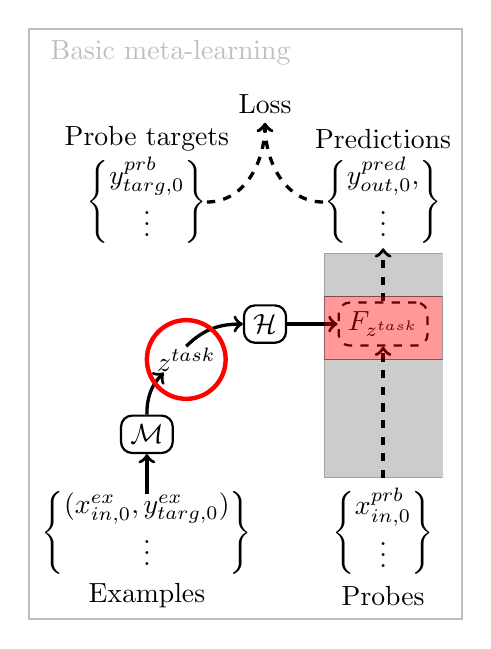
\begin{tikzpicture}
\draw[boundingbox, fill=white] (-3, -4.3) rectangle (2.5, 3.2);
\node[lightgray] at (-1.2, 2.9) {Basic meta-learning};
\node at (-1.5, -4) (examples) {Examples};
\node at (-1.5, -3.2) (D1) {
\(\left\{
\begin{matrix}
(x^{ex}_{in,0}, y^{ex}_{targ,0})\\
$\vdots$
\end{matrix}\right\}\)};

\node at (1.5, -4) (probes) {Probes};
\node at (1.5, -3.2) (D2) {
%\(z^{prb}_{in}\)};
\(\left\{
\begin{matrix}
x^{prb}_{in,0}\\
$\vdots$
\end{matrix}\right\}\)};

\node [block] at (-1.5, -1.95) (M) {\(\mathcal{M}\)};
\path [arrow] ([yshift=-5]D1.north) to (M);

\node at (-1, -1) (zfunc) {\(z^{task}\)};
\path [arrow, out=90, in=-135] (M.north) to ([xshift=6,yshift=3]zfunc.south west);

\node[block] at (0, -0.55) (H) {\(\mathcal{H}\)};
\path [arrow, out=45, in=180] ([yshift=-3]zfunc.north) to (H.west);
\node [block, dashed] at (1.5, -0.55) (F) {\(F_{z^{task}}\)};
\path[arrow] (H.east) to (F.west);
\path [arrow, dashed] (D2) to (F);

\node at (1.5, 1) (outputs) {
%\(z^{pred}_{out}\)};
\(\left\{
\begin{matrix}
y^{pred}_{out,0},\\
$\vdots$
\end{matrix}\right\}\)};
\node at (1.5, 1.8) (predictions) {Predictions};

\path [arrow, dashed] (F) to ([yshift=3]outputs.south);

\node at (-1.5, 1.8) (probetargs) {Probe targets};
\node at (-1.5, 1) (D2targs) {
%\(z^{prb}_{in}\)};
\(\left\{
\begin{matrix}
y^{prb}_{targ,0}\\
$\vdots$
\end{matrix}\right\}\)};

\node [align=center, text width=1.25 cm] at (0, 2.25) (dispatch) {\baselineskip=12pt Loss\par};

\path [arrow, dashed, out=180, in=-90] ([xshift=3]outputs.west) to (dispatch.south);

\path [arrow, dashed, out=0, in=-90] ([xshift=-3.5]D2targs.east) to (dispatch.south);

%% overlay

\draw [fill=black, opacity=0.2] (0.75, -0.2) rectangle (2.25, 0.35);
\draw [fill=red, opacity=0.4] (0.75, -1) rectangle (2.25, -0.2);
\draw [fill=black, opacity=0.2] (0.75, -2.5) rectangle (2.25, -1);

\uncover<4->{
\draw [red, ultra thick] (-1, -1) circle (0.5);
}
\end{tikzpicture}
\end{column}
\end{columns}

\end{frame}

\begin{frame}{Results}
\includegraphics[height=0.8\textheight]{figures/grids_adaptation.png}
\end{frame}

\begin{frame}[standout]
Meta-mapping works in RL, even with a small support set of tasks. 
\end{frame}

\begin{frame}{Relation to model-based adaptation}
Model-based methods are often framed in part as an approach to flexibility.
\begin{itemize}
\item However, for this to work, these methods generally must have a new reward function handed to them.
\item That is, they're offloading a substantial part of the adaptation problem to another system.
\item Meta-mapping offers a principled way to adapt a reward-predicting function, which a model-based system could then plan over.
\item It could also adapt transition models, e.g. when it starts raining and California drivers get confused. 
\item Thus meta-mapping and model-based planning could be complementary.
\end{itemize}
\end{frame}

\begin{frame}{Behavioral uncertainty}
\inlineMovie{figures/recording_pickup.mp4}{../../psych/dissertation/4-extending/figures/pick_up_0.png}{width=0.48\textwidth, height=0.36\textwidth}%
\inlineMovie{figures/recording_pusher.mp4}{../../psych/dissertation/4-extending/figures/pusher_0.png}{width=0.48\textwidth, height=0.36\textwidth}
\end{frame}


\begin{frame}{Categorization tasks}
\vspace{0.1em}
\begin{columns}
\begin{column}{\dimexpr\paperwidth-10pt}
\begin{tikzpicture}[auto]%, scale=0.8, every node/.style={scale=0.8}]
% blickets
\node at (-4.8, 2.2) {\LARGE ``Blickets''};
\draw[pen colour=fg, decoration={calligraphic brace, amplitude=0.5cm},decorate,line width=1mm] (-3, 0.3) -- (-3, 4); 
\node at (-2, 3.1) {\includegraphics[width=1.8cm]{../../psych/dissertation/4-extending/figures/categorization_stimuli/32_red_triangle_0.png}};
\node at (-2, 1.2) {\includegraphics[width=1.8cm]{../../psych/dissertation/4-extending/figures/categorization_stimuli/24_red_triangle_0.png}};

% not blickets
\node at (-4.3, -2.1) {\LARGE ``Not''};
\draw[pen colour=fg, decoration={calligraphic brace, amplitude=0.5cm},decorate,line width=1mm] (-3, -4) -- (-3, -0.3); 
\node at (-2, -3.1) {\includegraphics[width=1.8cm]{../../psych/dissertation/4-extending/figures/categorization_stimuli/32_red_circle_0.png}};
\node at (-2, -1.2) {\includegraphics[width=1.8cm]{../../psych/dissertation/4-extending/figures/categorization_stimuli/24_yellow_triangle_0.png}};
\only<2>{
\node at (1.3, 0) {\LARGE ``Blickets?''};
}
\uncover<3->{
\node at (3, 3.5) {\LARGE ``Zipfs = cyan blickets''};
\node at (1.6, 0) {\LARGE ``Zipfs?''};
}
\uncover<2->{
\draw[pen colour=fg, decoration={calligraphic brace, amplitude=0.5cm},decorate,line width=1mm] (3.2, -2.9) -- (3.2, 2.9); 
\node at (4.2, 1.9) {\includegraphics[width=1.8cm]{../../psych/dissertation/4-extending/figures/categorization_stimuli/24_red_triangle_1.png}};
\node at (4.2, 0) {\includegraphics[width=1.8cm]{../../psych/dissertation/4-extending/figures/categorization_stimuli/32_cyan_triangle_1.png}};
\node at (4.2, -1.9) {\includegraphics[width=1.8cm]{../../psych/dissertation/4-extending/figures/categorization_stimuli/32_cyan_inverseplus_1.png}};
}

\end{tikzpicture}
\end{column}
\end{columns}
\end{frame}


\begin{frame}{Why categorization?}
\begin{itemize}
\item Cognitive history.
\item Rich visual input, more complex tasks.
\item Classification is a common problem.
\end{itemize}
\end{frame}
\begin{frame}{Categorization tasks}
\begin{columns}
\begin{column}{0.5\textwidth}
Types of categories:
\begin{itemize}
\item Basic tasks: single attribute (shape/color/size) category.
\item Composite tasks: AND, OR, or XOR of two different attributes.  
\end{itemize}
\uncover<2->{
Meta-mappings:
\begin{itemize}
\item Switch one color to another or switch one shape to another. 
\item (Omitted size switching because only a few sizes.)
\end{itemize}
}
\end{column}
\begin{column}{0.5\textwidth}
\centering
\includegraphics[width=2.2cm]{../../psych/dissertation/4-extending/figures/categorization_stimuli/24_red_triangle_1.png}\\
\includegraphics[width=2.2cm]{figures/categorization/32_cyan_emptysquare_0.png}\\
\includegraphics[width=2.2cm]{../../psych/dissertation/4-extending/figures/categorization_stimuli/24_yellow_inverseplus_0.png}
\end{column}
\end{columns}
\end{frame}

\againframe<2>{extending_methods}

\begin{frame}<1>[label=cat_results]
\frametitle{Categorization results}
\only<1>{
\includegraphics[height=0.8\textheight]{figures/categories_adaptation_no_lh.png}
}
\only<2>{
\includegraphics[height=0.8\textheight]{figures/categories_adaptation.png}
}
\end{frame}

\againframe<4>{homm_arch}
\againframe<2>{cat_results}

\begin{frame}[standout]
Language produces better concept representations than examples.\\[1em]
Meta-mapping these representations produces similar performance to langauge generalization.
\end{frame}

\begin{frame}{Thoughts on language \& my recent RL generalization work}
How does this relate to our recent finding that realistic tasks improve generalization in language-conditioned RL?\par
\begin{itemize}[<+(1)->]
\item In some cases this approach appears to be quite sample efficient, e.g. only 16 training tasks in RL.
\item This is despite having \textbf{more challenging} evaluation than the language work, since often the adapted task \textbf{contradicts previous learning} (e.g. was negatively rewarded). 
\item Language does seem to be a better way of constructing task representations in the categorization setting, where there were many more training tasks, with language + meta-mapping adapting similarly to language generalization. 
\item Whether this perspective is computationally useful with data as rich as human experience is an open question.
\end{itemize}
(``Environmental drivers of generalization in a situated agent,'' Hill, Lampinen, et al., ICLR 2020)
\end{frame}

\section{Interactions with other timescales of learning}

\begin{frame}{Why do zero-shot adaptation?}
Because it accelerates learning and reduces cumulative mistakes.
{
\centering
\only<1>{
\includegraphics[height=0.8\textheight]{../../psych/dissertation/5-timescales/figures/polynomial_optimization_curves.png}
}
\only<2>{
\includegraphics[height=0.8\textheight]{../../psych/dissertation/5-timescales/figures/polynomial_optimization_cumulative_regret.png}
}
}
\end{frame}

\begin{frame}[standout]
Starting from a zero-shot ``guess'' at the appropriate behavior results in faster learning, and reduces cumulative mistakes by an order of magnitude 
\end{frame}


\section{Wrapping up}

\begin{frame}{Conclusions}

\begin{itemize}
\item Humans can perform novel tasks zero-shot. 
\item We suggest a computational perspective on this: \textbf{meta-mappings} -- functions which map a task to a transformed version of that task. 
\item We propose a parsimonious \textbf{HoMM} architecture that: 
    \begin{itemize}
    \item Performs basic tasks by parameterizing a small task network from a vector representation of the task. 
    \item Uses an analogy between basic tasks and meta-mappings to perform meta-mappings by transforming task embeddings. 
    \end{itemize}
\item This approach performs comparably to humans in a card game task, and outperforms (or equals) a language based approach across three settings.
\item Zero-shot adaptation allows faster, better later learning. 
\item Earlier paper: \url{https://arxiv.org/abs/1905.09950} and library + all code: \url{https://github.com/lampinen/HoMM}
\end{itemize}
\end{frame}

\section{A brief methods comment}
\begin{frame}{Why you should implement everything twice}
\only<1>{
Bugs that slipped past my unit testing, but that I found by reimplementing my code in a shared library, and comparing results:%
\begin{itemize}
\item Off-by-one error in array indexing leading to unintentional, weird weight tying in hyper network output. 
\item Target network for DQN accidentally having one set of weights shared with main net all the time.
\item Using mixed task representations for evaluation rather than cached ones in RL tasks.
\item Error in domains of meta-mappings in categorization tasks.
\item Implementation of suit \(\leftrightarrow\) rank in card tasks not as intended.
\end{itemize}
None of these made my earlier results invalid, but they did worsen performance in some cases, and/or made it so I wasn't really doing what I thought/said I was. All results I showed you today are from the corrected version.
}
\only<2>{
But I was lucky:\\
\includegraphics[width=\textwidth]{figures/correction.png}
}
\end{frame}

\begin{frame}[standout]
Thanks to Jay, Noah, Surya, Erin, Katherine, Arianna and the rest of the lab! \\[1em]
And you for listening! \\[1em]
Questions?
\end{frame}

\end{document}
